\begin{enumerate}[label=\thesection.\arabic*.,ref=\thesection.\theenumi]
\numberwithin{equation}{enumi}

\begin{frame}
   A lead Compensator network includes a parallel combination of R and C in feed-forward path. If the transfer function of compensator  is $$G_c(s) = \frac{s+2}{s+4}$$, the value of RC is ?\\
\begin{figure}{t}
    \graphicspath{{./images/}}
    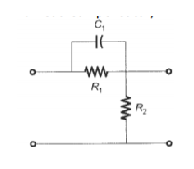
\includegraphics{figs/circuit_lead_compensator.eps}{}
    \centering
    \par
This is the circuit of lead compensator with parallel RC combination.
\end{figure}
Solution:\\
The transfer function for the following circuit is
    $$
    T(s) = \frac{V_o}{V_i}
    $$
    Let
    $$
    \alpha = \frac{R_2}{R_1 + R_2}
    $$
    and 
    $$
    \tau = R_1C
    $$

Now our T(s) is 
    $$
    T(s) = \frac{R_2}{\frac{\frac{1}{sC}R1}{\frac{1}{sC}+R1} + R2}
    $$
    Simplifying T(s)
    $$
    T(s) = \frac{s+\frac{1}{\tau}}{s+\frac{1}{\tau\alpha}}
    $$
    Comparing with the given $$G_c(s) = \frac{s+2}{s+4}$$
    $$
    \tau = R_1C = 0.5
    $$
\end{frame}

\end{enumerate}
